\documentclass[10pt, letterpaper]{article}
\usepackage[utf8]{inputenc}
\usepackage{amsmath}
\usepackage{amssymb}
\usepackage{bbm}
\usepackage{booktabs}
\usepackage{caption}
\usepackage{color}
\usepackage[shortlabels]{enumitem}
\usepackage{fancyhdr}
\usepackage{hyperref}
\usepackage{geometry}
\geometry{a4paper,scale=0.8}
\usepackage{graphicx}
\graphicspath{ {./img/}}
\usepackage{listings}
\usepackage{mathtools}
\usepackage{mathrsfs}
\usepackage{setspace}
\renewcommand{\baselinestretch}{1.3}

% set-up header & footer
\pagestyle{empty}
\fancyhf{}
\cfoot{\thepage}
\lhead{%
\textbf{University of California, Berkeley} \\
Department of Civil \& Environ. Eng.
}
\rhead{\textbf{CS 285 Deep Reinforcement Learning}\\\date{\today}}

\title{%
    \textbf{Homework 3}
}
\author{Juanwu Lu (3037432593)\\ \small(M.Sc. Civil Engineering, UC Berkeley)}
\date{}

% set-up code listing
\definecolor{dkgreen}{rgb}{0,0.6,0}
\definecolor{gray}{rgb}{0.5,0.5,0.5}
\definecolor{manuve}{rgb}{0.58,0,0.82}

\lstset{frame=tb,
    language=Python,
    aboveskip=3mm,
    belowskip=3mm,
    showstringspaces=false,
    columns=flexible,
    basicstyle={\small\ttfamily},
    numbers=none,
    numberstyle=\tiny\color{gray},
    keywordstyle=\color{blue},
    commentstyle=\color{dkgreen},
    stringstyle=\color{manuve},
    breaklines=true,
    breakatwhitespace=true,
    tabsize=3
}

\begin{document}
\maketitle
\captionsetup[figure]{labelfont={bf},labelformat={default},labelsep=period,name={Figure}}
\captionsetup[table]{labelfont={bf},labelformat={default},labelsep=period,name={TABLE}}
\thispagestyle{fancy}
\pagestyle{plain}

% Part 1: Q-Learning
\section{Part 1: Q-Learning}

\subsection*{Question 1: basic Q-learning performance (DQN)}
\subsubsection*{Results}
\begin{figure}[thbp]
    \centering
    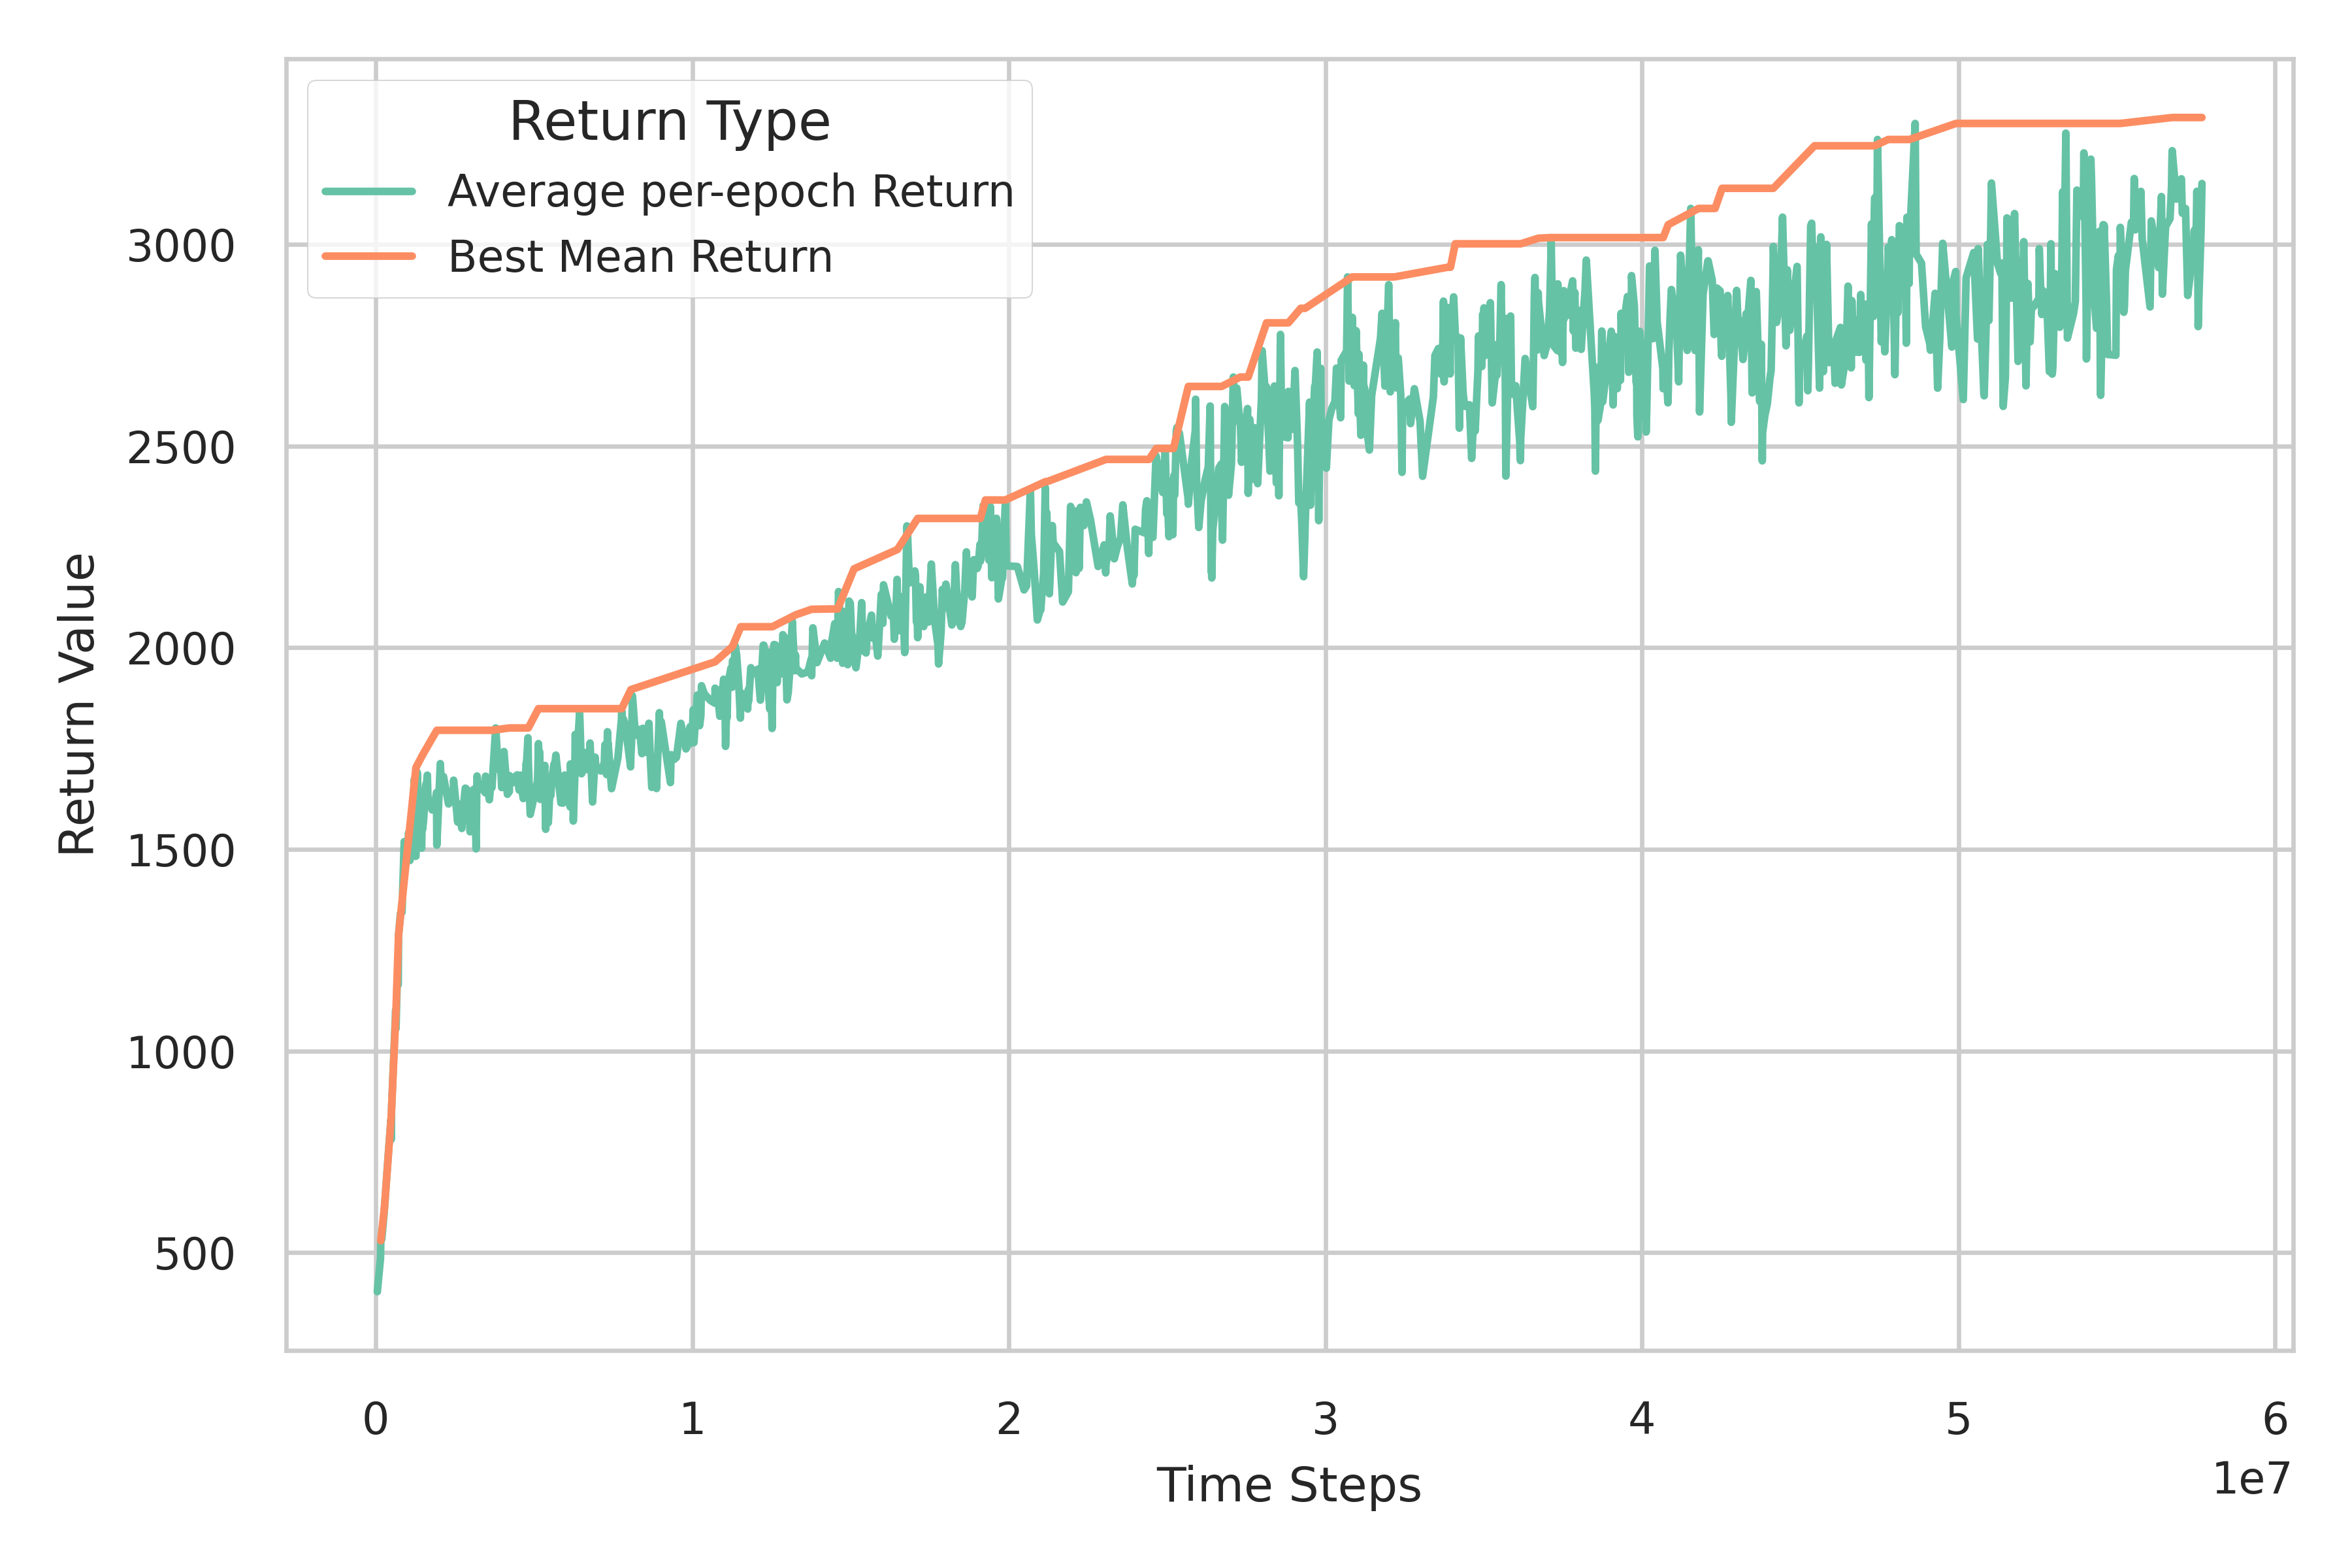
\includegraphics[width=\textwidth]{./img/q1.png}
    \caption{DQN performance on \texttt{Ms. Pac-Man} in average per-epoch return (cyan curve) and best mean return (red curve) versus number of time steps. Performance of the algorithm shows a step increasing trend. However, the average per-epoch return variances are also increasing.}
    \label{fig:1}
\end{figure}
\subsubsection*{Codes}
\begin{lstlisting}
    python cs285/scripts/run_hw3_dqn.py --env_name MsPacman-v0 --exp_name q1 -gpu_id $1
\end{lstlisting}

\pagebreak
\subsection*{Question 2: double Q-learning (DDQN)}
\subsubsection*{Results}
\begin{figure}[thbp]
    \centering 
    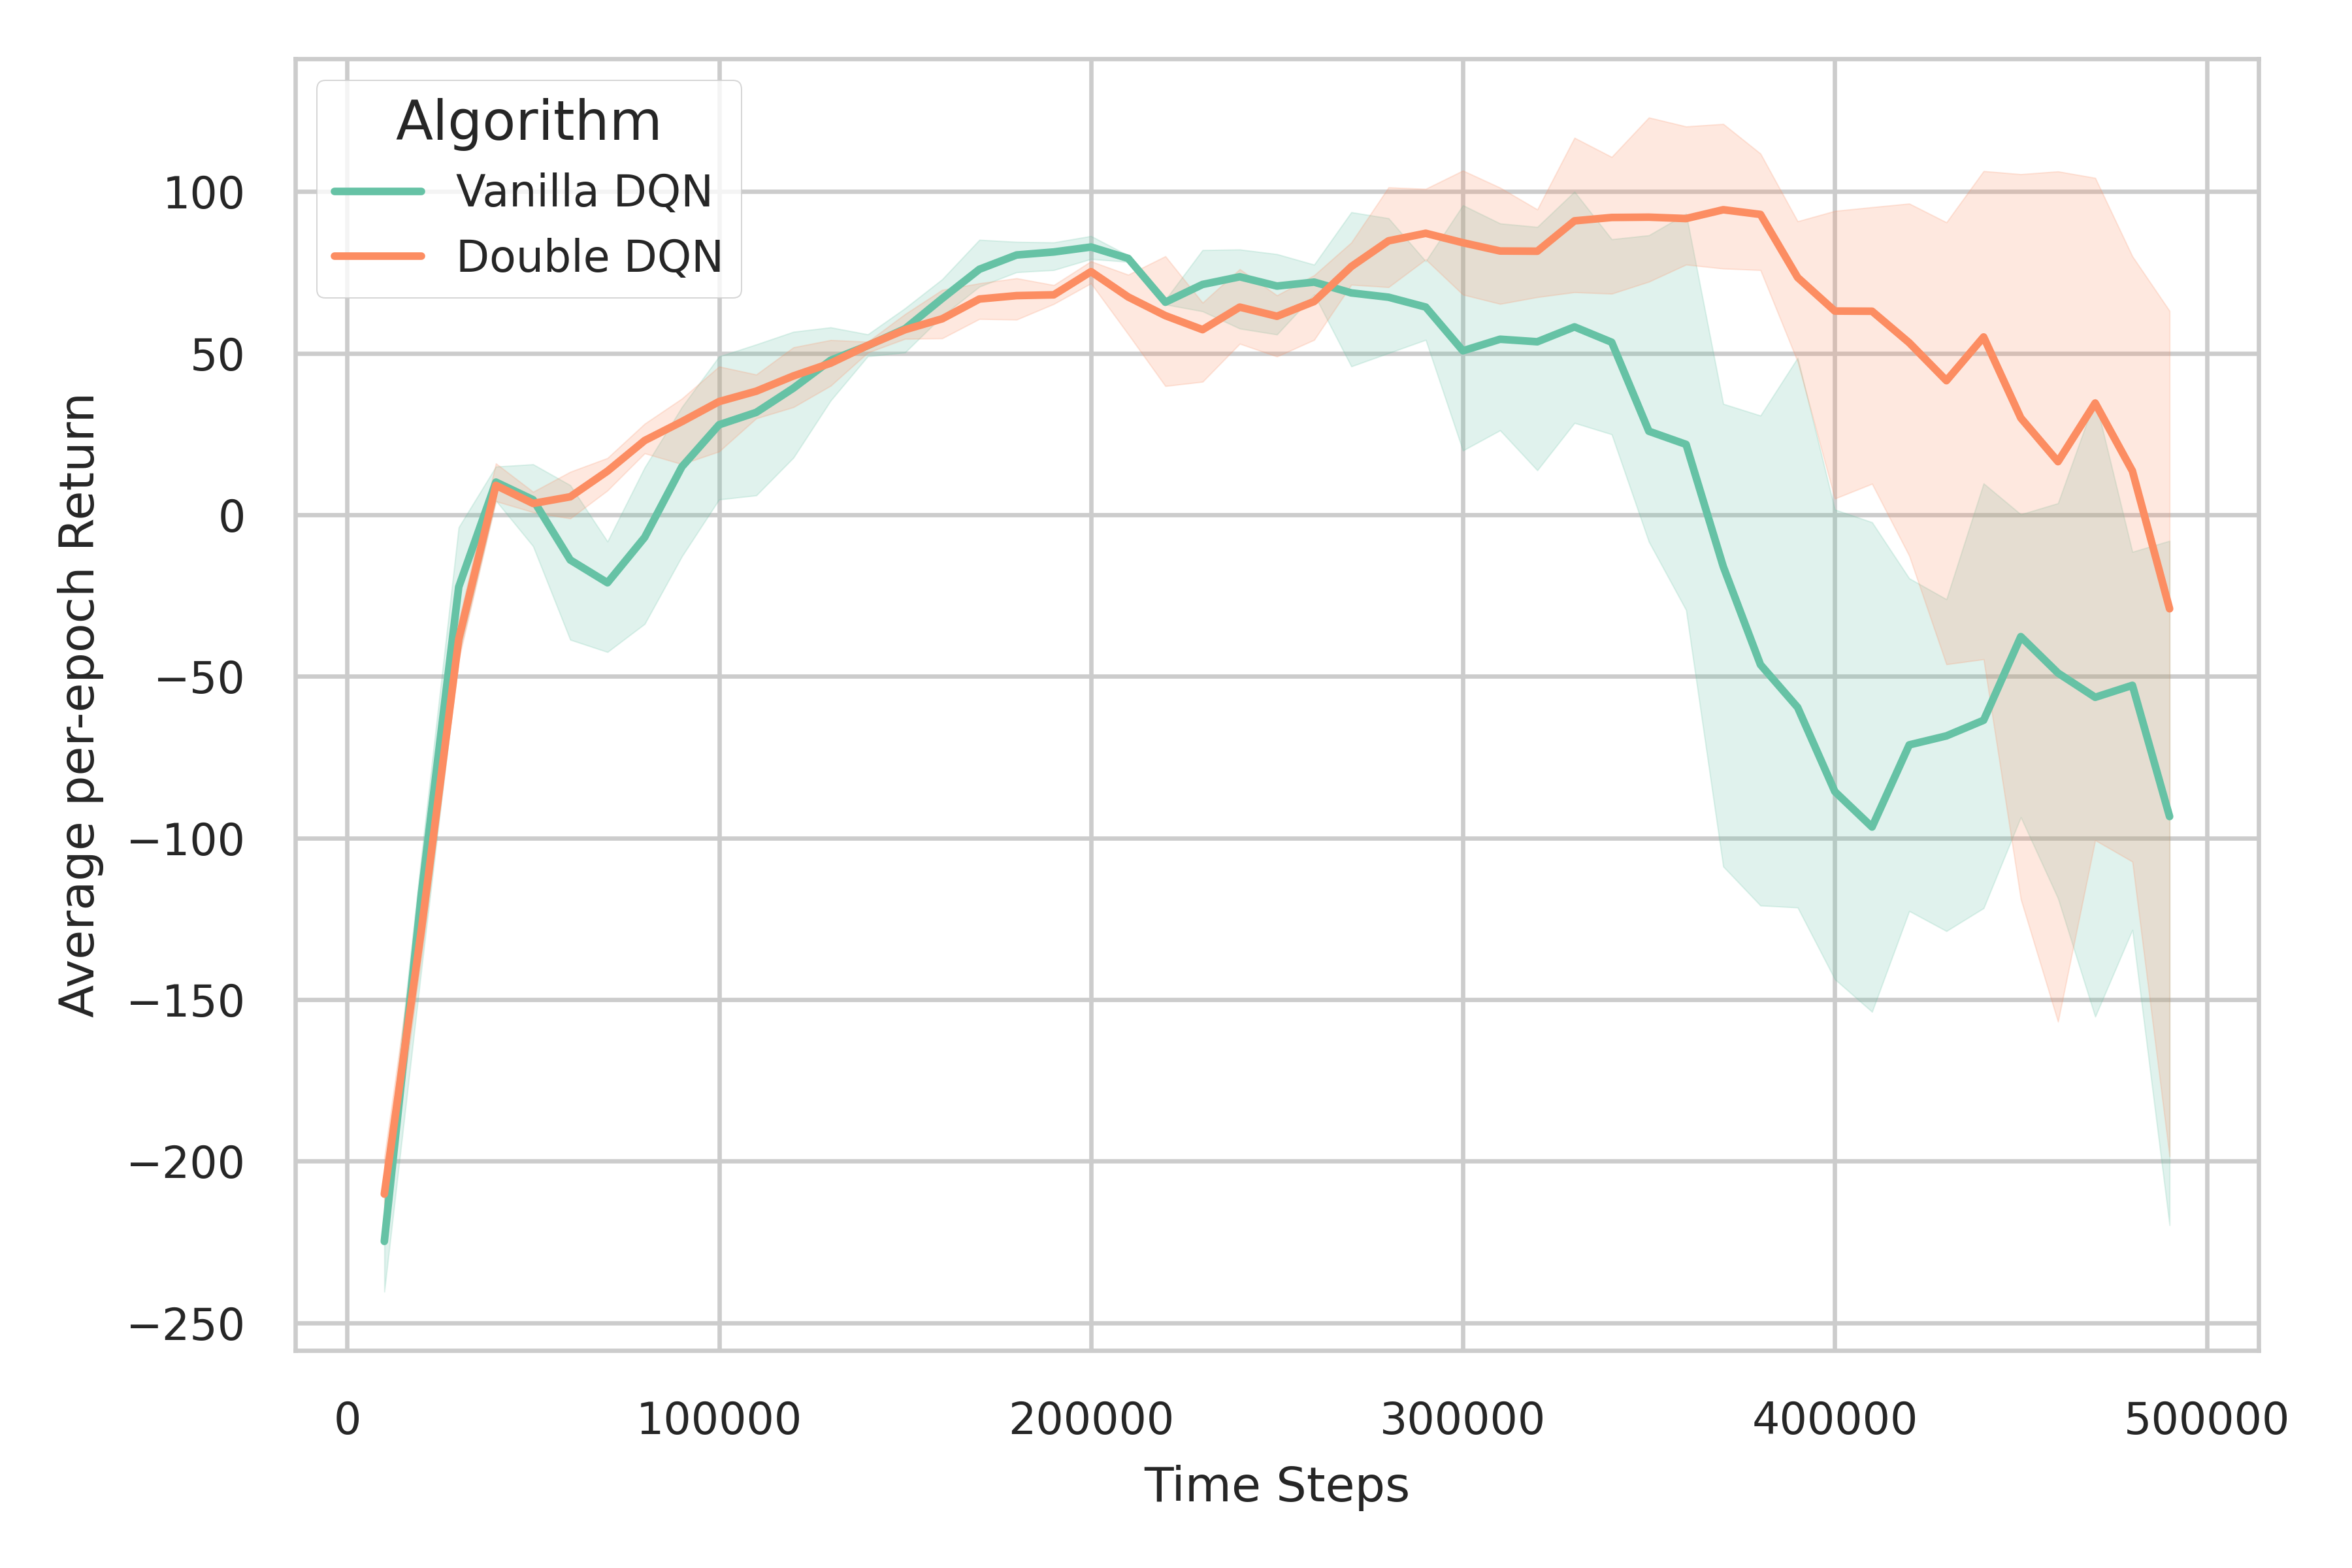
\includegraphics[width=\textwidth]{./img/q2.png}
    \caption{Average training per-epoch return with respect to vanilla (green curve) and double (orange curve) DQN. The double DQN successfully prevents rewards from decreasing after around $30,000$ training steps and achieves a higher score.}
    \label{fig:2}
\end{figure}
\subsubsection*{Codes}
\begin{lstlisting}
    echo "Running Homework 3 Question 2";
    python $1 --env_name LunarLander-v3 --exp_name q2_dqn_1 --seed 1 -gpu_id $2;
    python $1 --env_name LunarLander-v3 --exp_name q2_dqn_2 --seed 2 -gpu_id $2;
    python $1 --env_name LunarLander-v3 --exp_name q2_dqn_3 --seed 3 -gpu_id $2;

    python $1 --env_name LunarLander-v3 --exp_name q2_doubledqn_1 --double_q --seed 1 -gpu_id $2;
    python $1 --env_name LunarLander-v3 --exp_name q2_doubledqn_2 --double_q --seed 2 -gpu_id $2;
    python $1 --env_name LunarLander-v3 --exp_name q2_doubledqn_3 --double_q --seed 3 -gpu_id $2;
    echo "Question 2 Done!"
\end{lstlisting}

\pagebreak
\subsection*{Question 3: experimenting with hyperparameters}
\subsubsection*{Results}

For this question I explore the influence of different \texttt{hidden\_size} settings of the Q-function network on the training process. Intuitively, higher number of neurons yields better ability to represent non-linear relationships, which explains why performance under \texttt{hparam3} are lower compared to the others at the earlier stage of the training. But with sufficient training, all network structures converge to a similar performance level.

\begin{figure}[thbp]
    \centering
    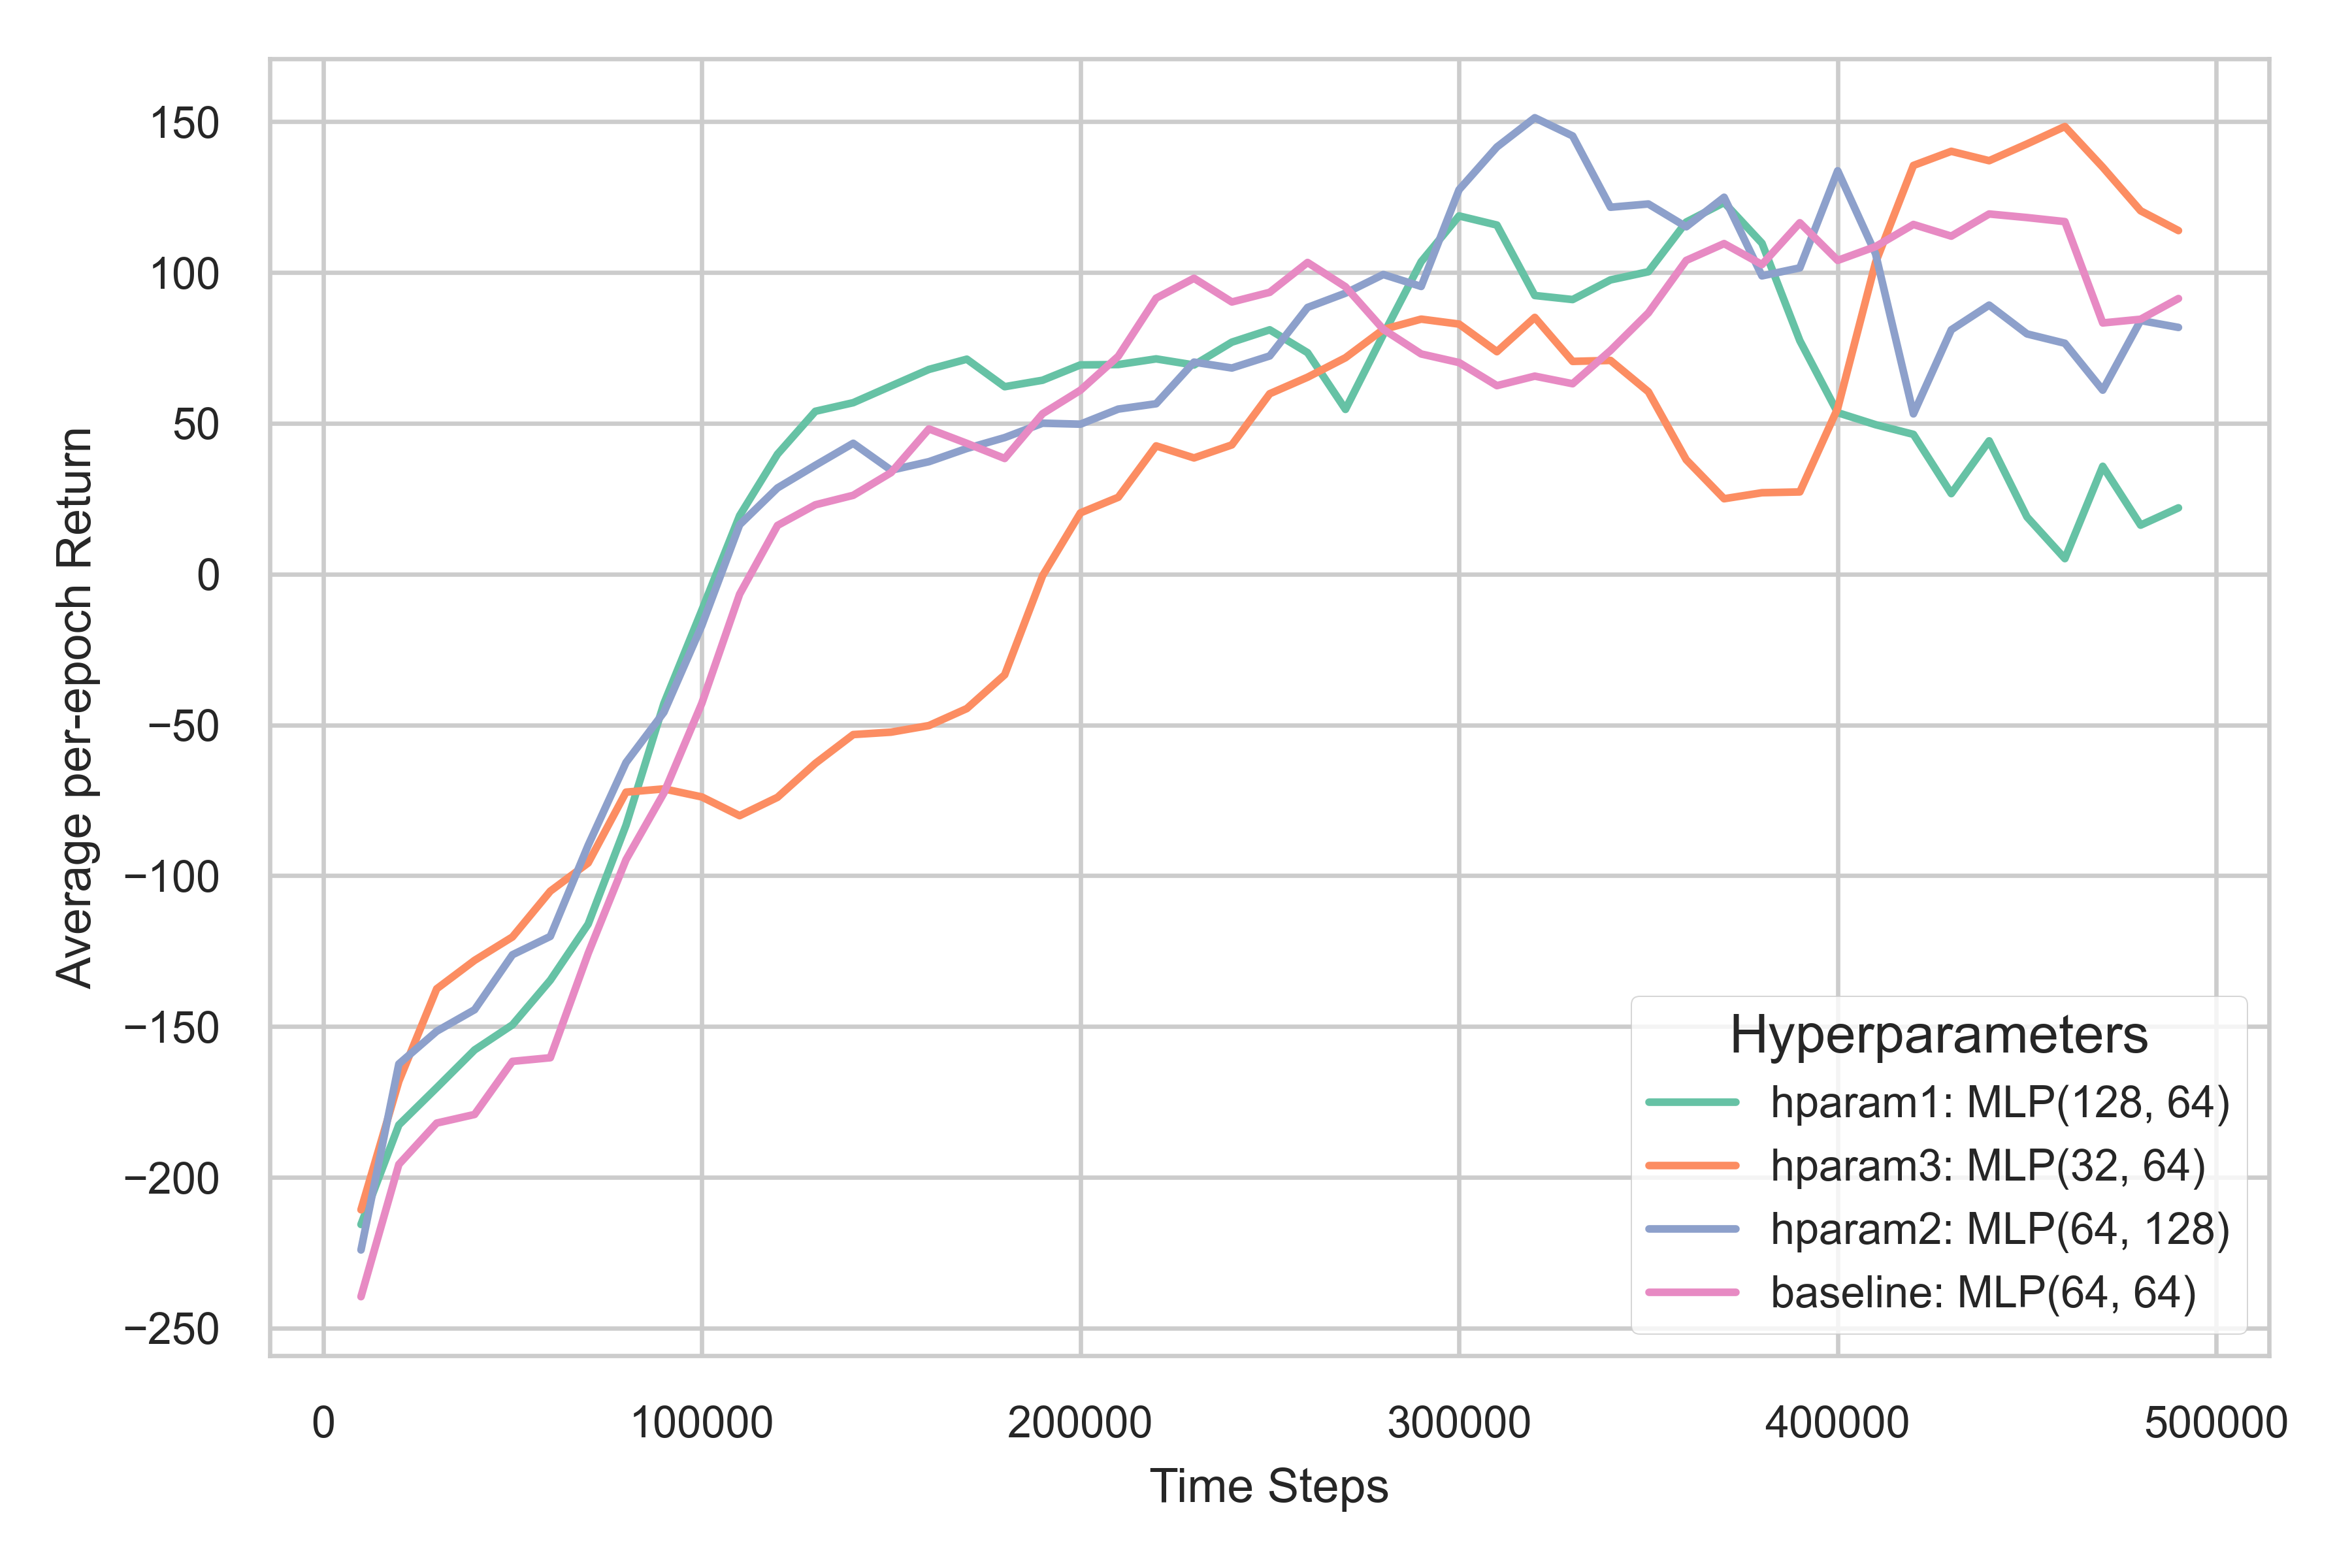
\includegraphics[width=\textwidth]{q3.png}
    \caption{Average per-epoch training returns with respect to training time steps given different Q-function neural network structures.}
    \label{fig:3}
\end{figure}
\subsubsection*{Codes}
\begin{lstlisting}
    python cs285/scripts/run_hw3_dqn.py --env_name LunarLander-v3 --exp_name q3_hparam1 -gpu_id $1;
    python cs285/scripts/run_hw3_dqn.py --env_name LunarLander-v3 --exp_name q3_hparam2 -gpu_id $1;
    python cs285/scripts/run_hw3_dqn.py --env_name LunarLander-v3 --exp_name q3_hparam3 -gpu_id $1;
\end{lstlisting}

% figure

% Part 2: Actor-Critic
\newpage
\section{Part 2: Actor-Critic}

\subsection*{Question 4: sanity check with \texttt{Cartpole-v0}}
\subsubsection*{Results}
\begin{figure}[thbp]
    \centering
    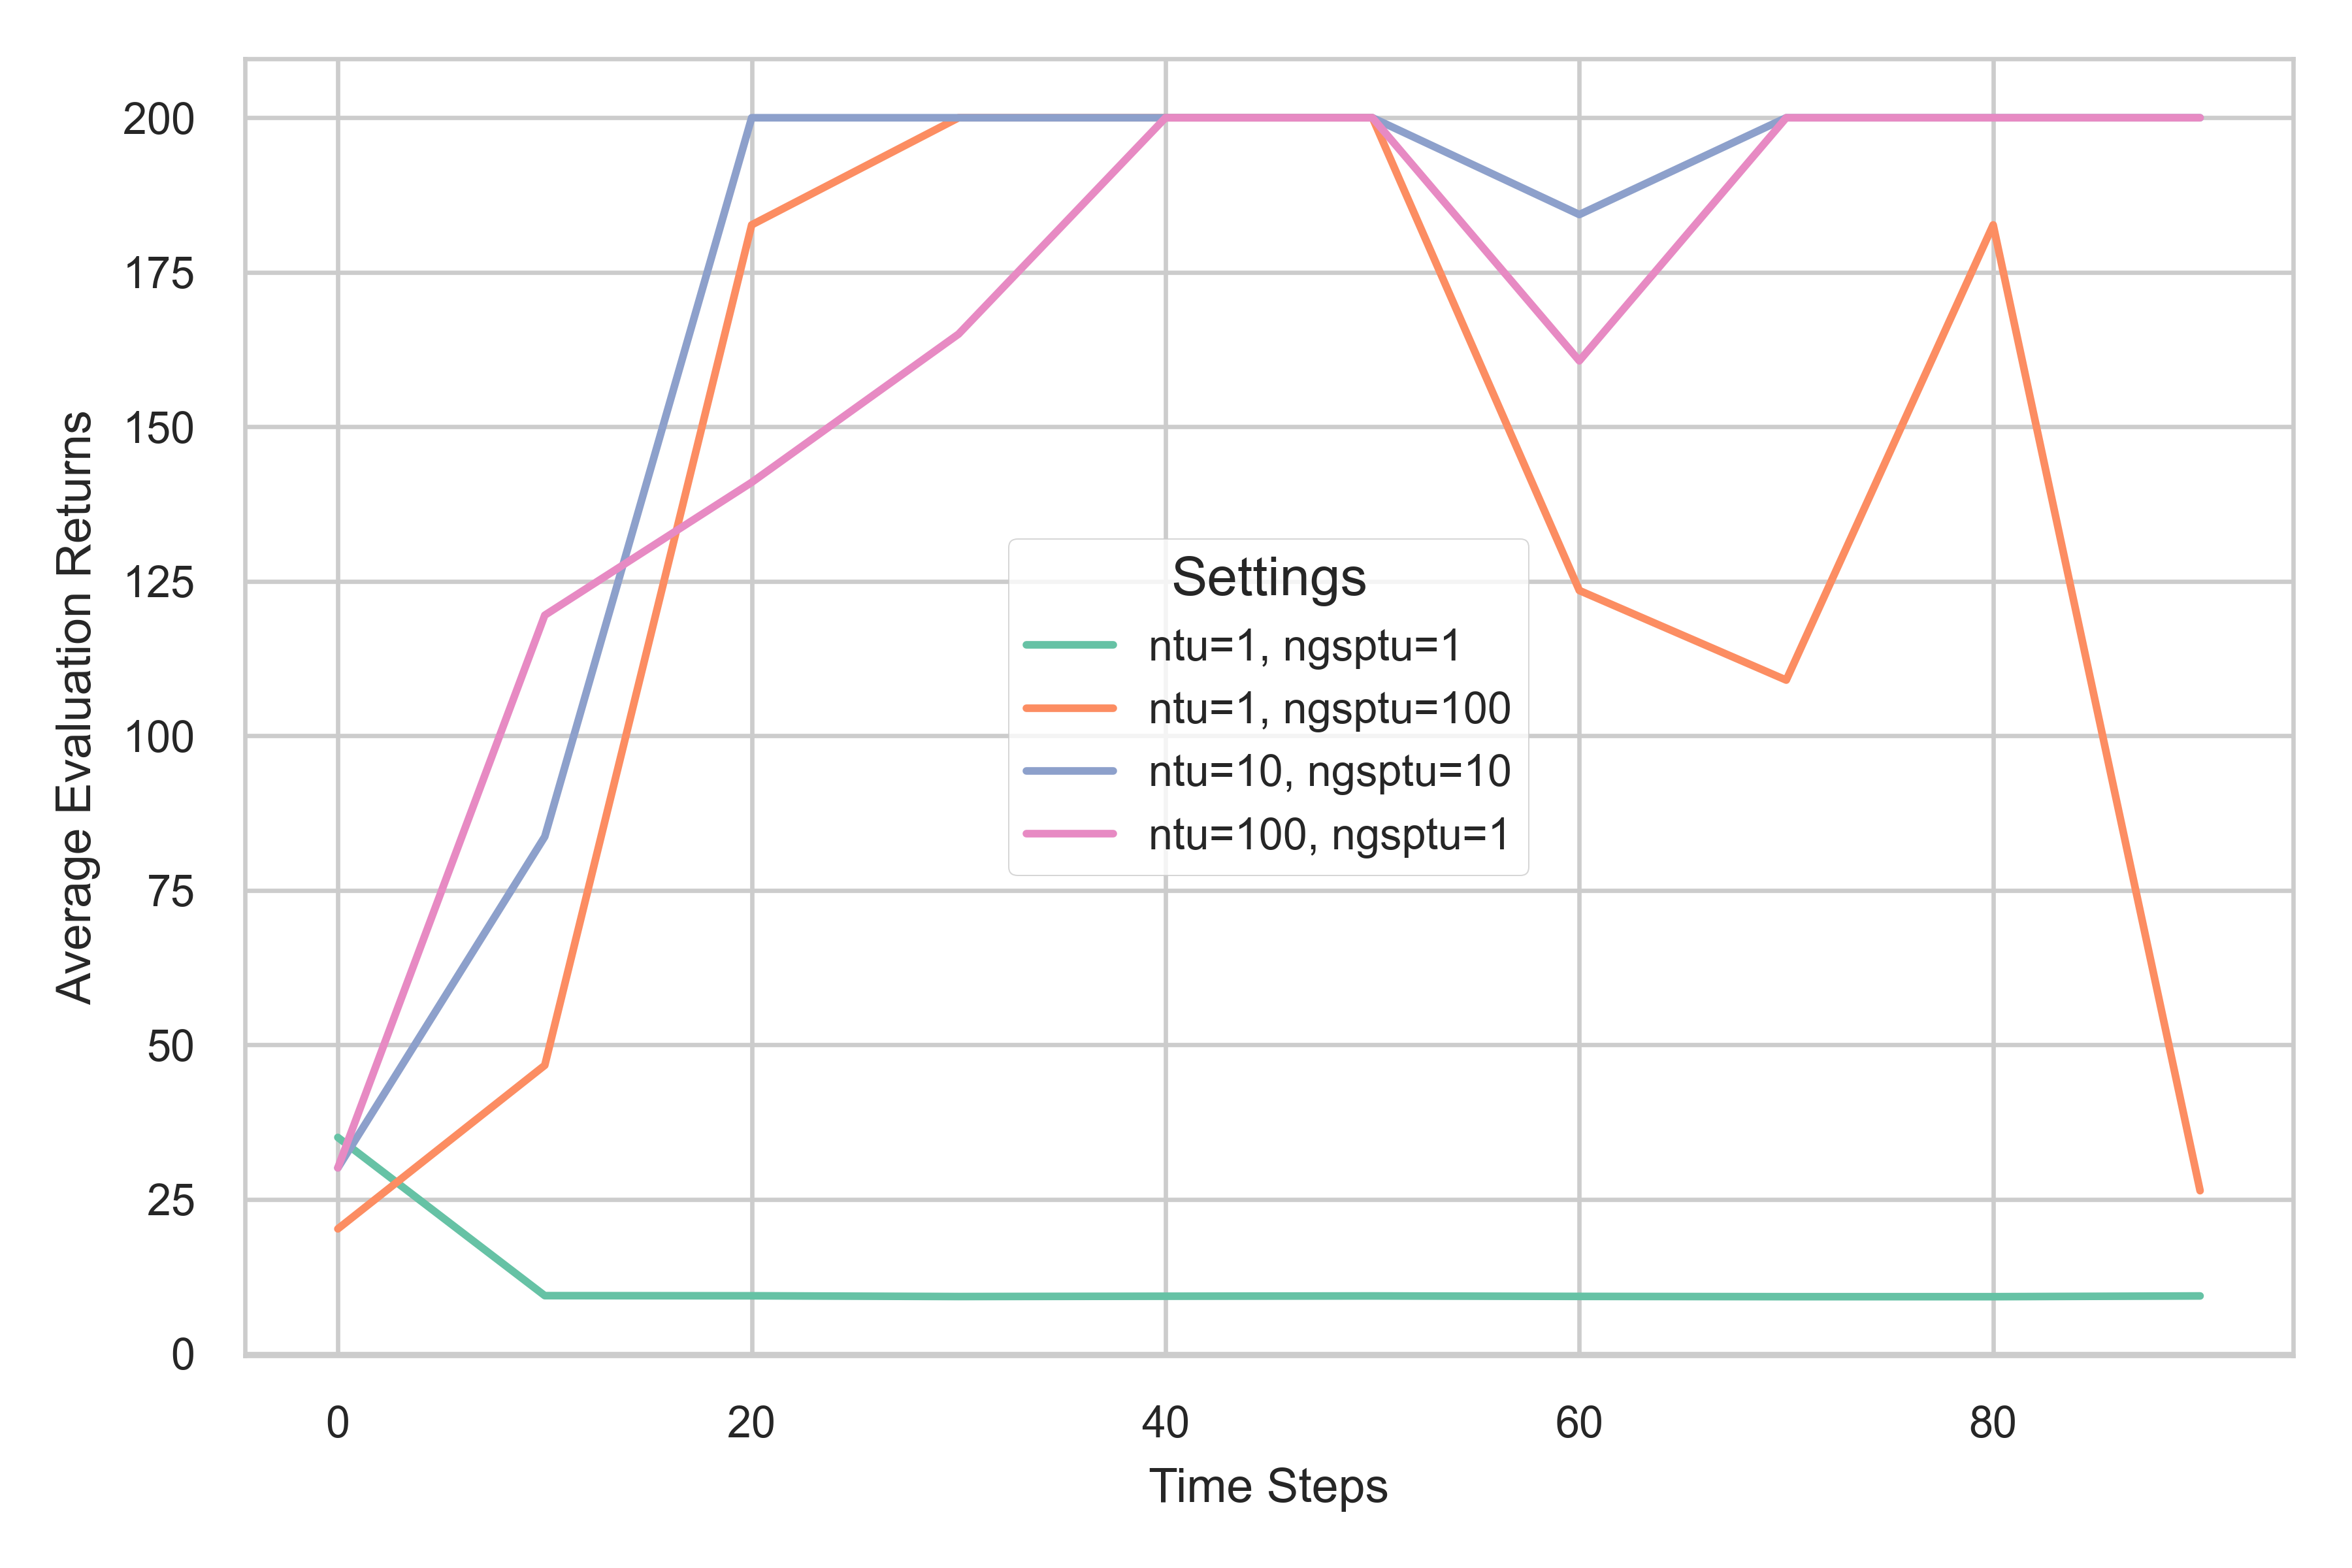
\includegraphics[width=\textwidth]{img/q4.png}
    \caption{Average evaluation returns with respect to training time steps given different \texttt{ntu} and \texttt{ngsptu} settings. From the results, $10$ target updates along with $10$ gradient steps per target update yields the best results among the four different settings.}
    \label{fig:4}
\end{figure}
\subsubsection*{Codes}
\begin{lstlisting}
    echo "Running Homework 3 Question 4..."
    python $1 --env_name CartPole-v0 -n 100 -b 1000 --exp_name q4_ac_1_1 -ntu 1 -ngsptu 1 -gpu_id $2
    python $1 --env_name CartPole-v0 -n 100 -b 1000 --exp_name q4_ac_100_1 -ntu 100 -ngsptu 1 -gpu_id $2
    python $1 --env_name CartPole-v0 -n 100 -b 1000 --exp_name q4_ac_1_100 -ntu 1 -ngsptu 100 -gpu_id $2
    python $1 --env_name CartPole-v0 -n 100 -b 1000 --exp_name q4_ac_10_10 -ntu 10 -ngsptu 10 -gpu_id $2
    echo "Done!"
\end{lstlisting}

\pagebreak
\subsection*{Question 5: Run Actor-Critic with more difficult tasks}
\subsubsection*{Results}

\begin{figure}[thbp]
    \centering
    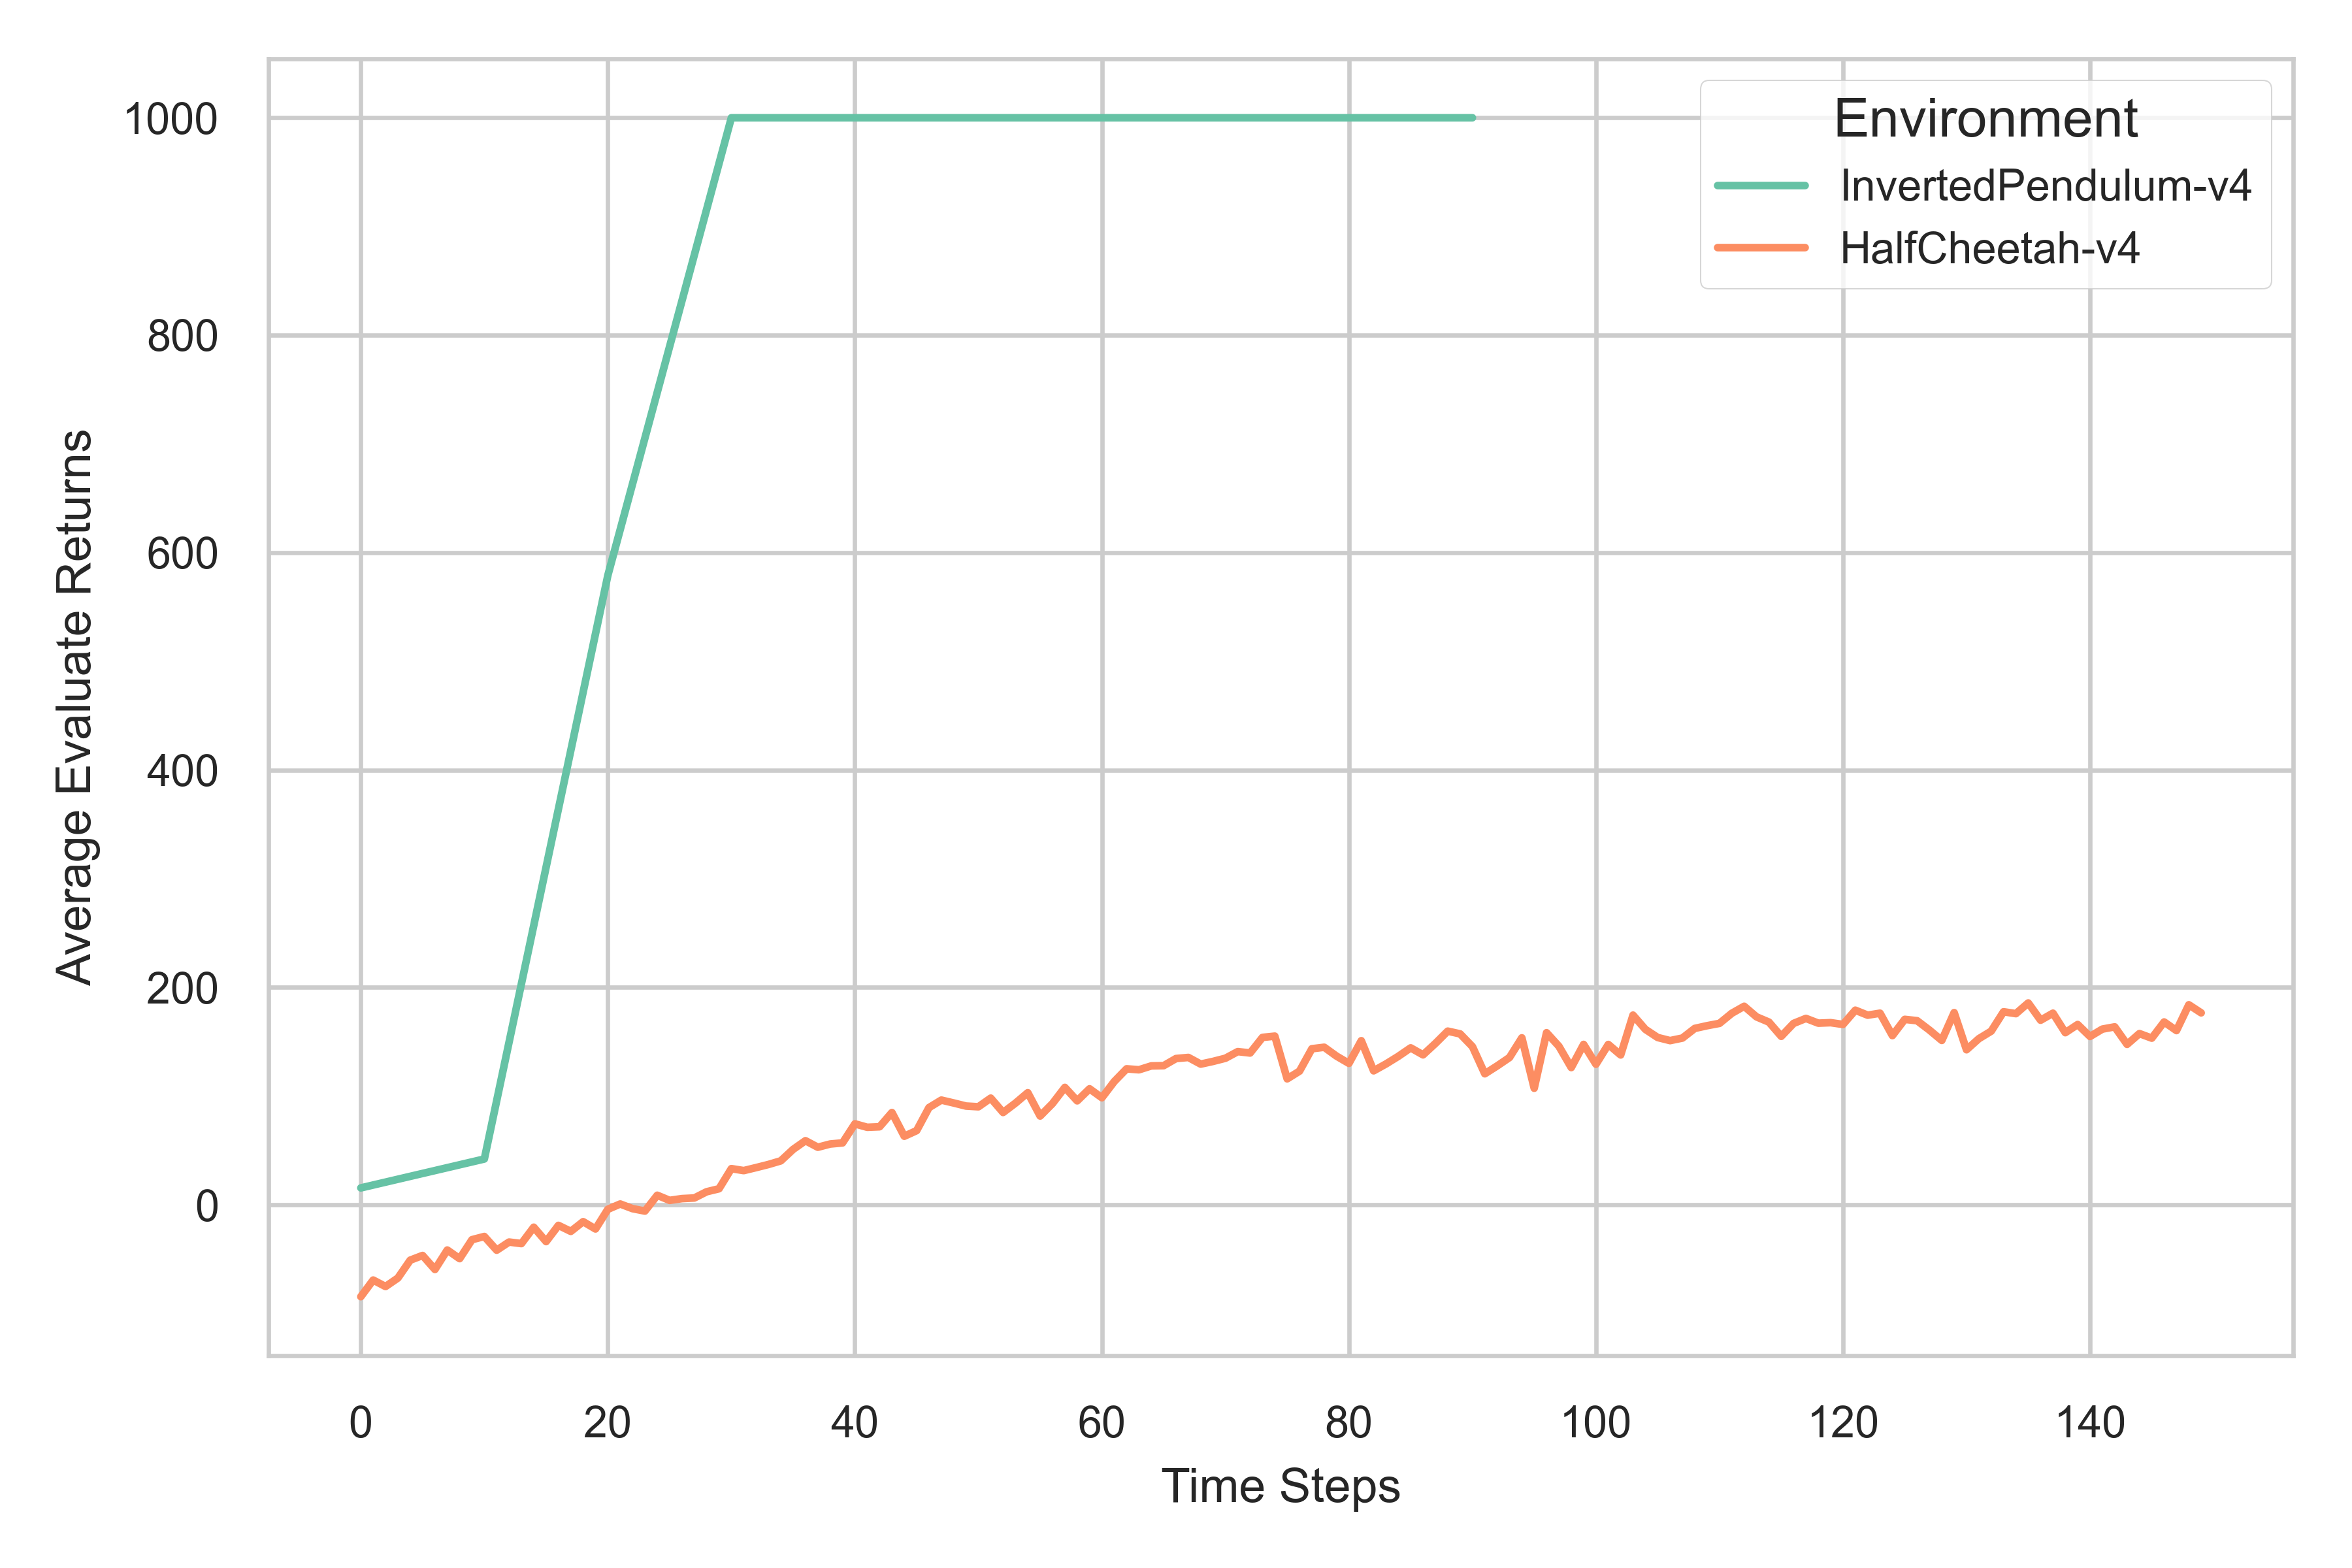
\includegraphics[width=\textwidth]{img/q5.png}
    \caption{Average evaluation return with respect to training steps of running Actor-Crtic algorithm with \texttt{InvertedPendulum-v4} (green) and \texttt{HalfCheetah-v4} (orange).}
    \label{fig:5}
\end{figure}
\subsubsection*{Codes}
\begin{lstlisting}
    NTU=$2
    NGSPTU=$3
    GPUID=$4

    echo "Running Homework 3 Question 5";
    python $1 --env_name InvertedPendulum-v4 --ep_len 1000 --discount 0.95 -n 100 -l 2 -s 64 -b 5000 -lr 0.01 --exp_name q5_${NTU}_${NGSPTU} -ntu $NTU -ngsptu $NGSPTU -gpu_id $GPUID;
    python $1 --env_name HalfCheetah-v4 --ep_len 150 --discount 0.90 --scalar_log_freq 1 -n 150 -l 2 -s 32 -b 30000 -eb 1500 -lr 0.02 --exp_name q5_${NTU}_${NGSPTU} -ntu $NTU -ngsptu $NGSPTU -gpu_id $GPUID
    echo "Done!"
\end{lstlisting}

% Part 3: Soft Actor-Critic
\newpage
\section{Part 3: Soft Actor-Critic}

\subsection*{Question 6: Run Soft Actor-Critic with more difficult tasks}
\subsubsection*{Results}
\begin{figure}[thbp]
    \centering 
    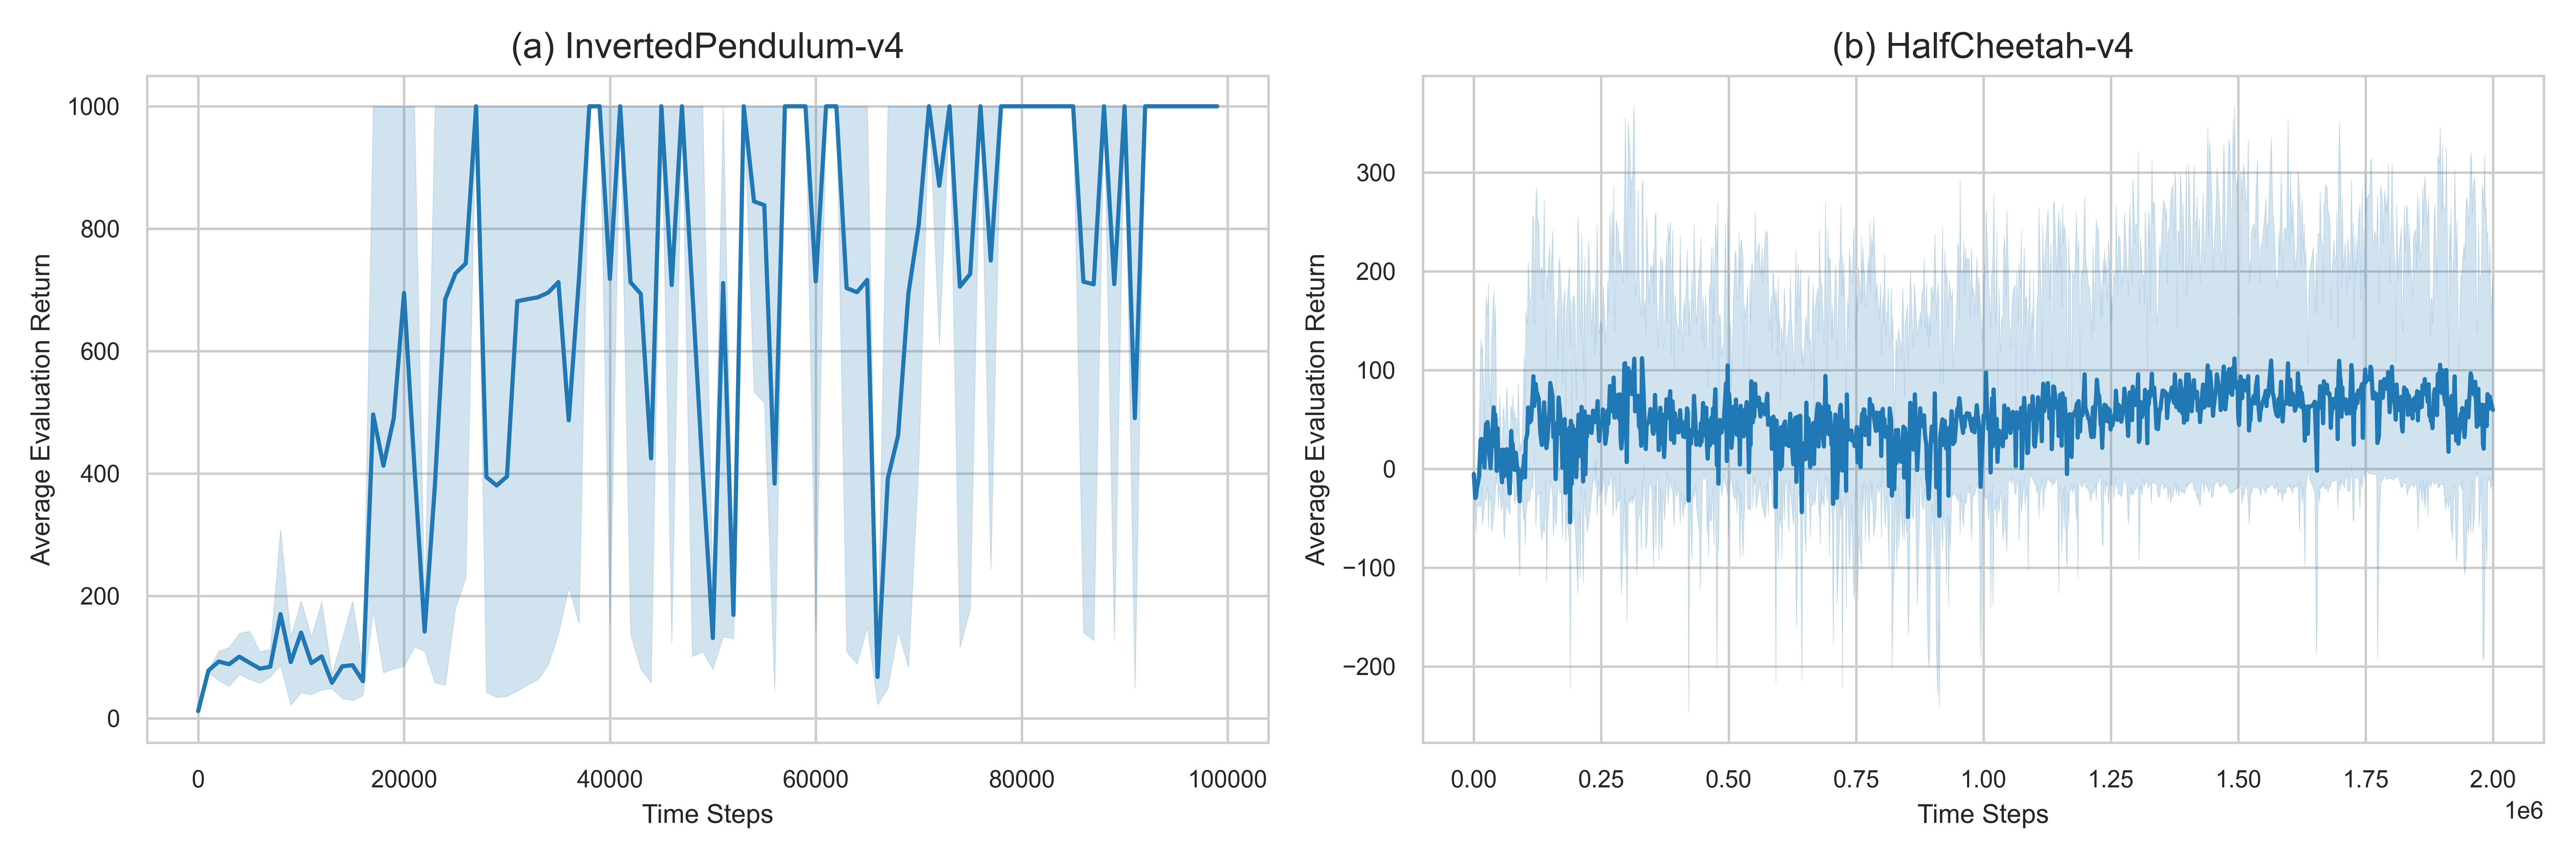
\includegraphics[width=\textwidth]{img/q6.png}
    \caption{Average Evaluation Returns running Soft Actor-Critic on \texttt{HalfCheetah-v4} (left) and \texttt{InvertedPendulum-v4} (right). Average rewards on \texttt{HalfCheetah-v4} reaches around $200$ after 50,000 steps, and rewards on \texttt{InvertedPendulum-v4} reaches $1,000$ after 20,000 steps. However, rewards on the second environment oscillate drastically indicating a potential high variance estimation of the state-value function.}
    \label{fig:6}
\end{figure}
\subsubsection*{Codes}
\begin{lstlisting}
    echo "Running Homework 3 Question 6";
    python cs285/scripts/run_hw3_sac.py --env_name InvertedPendulum-v4 --ep_len 1000 --discount 0.99 --scalar_log_freq 1000 -n 100000 -l 2 -s 256 -b 1000 -eb 2000 -lr 0.0003 --init_temperature 0.1 ----exp_name q6a_sac_InvertedPendulum_<parameters> --seed 1 -gpu_id $1;
    python cs285/scripts/run_hw3_sac.py --env_name HalfCheetah-v4 --ep_len 150 --discount 0.99 --scalar_log_freq 1500 -n 2000000 -l 2 -s 256 -b 1500 -eb 1500 -lr 0.0003 --init_temperature 0.1 --exp_name q6b_sac_HalfCheetah_<parameters> --seed 1 -gpu_id $1
    echo "Done!"
\end{lstlisting}

\end{document}